
\documentclass[twocolumn,10pt]{article}
\title{Constructing triangles}
\setlength{\columnsep}{20pt} 
\usepackage{amsmath,hyperref,cancel,graphicx}
 \def\shrinkfactor{0.45}
 \usepackage[margin=1.5cm]{geometry}
\usepackage[usenames,dvipsnames]{color}
 
 \newcommand{\blue}[1]{{\color{Blue}#1}} 
 \newcommand{\purple}[1]{{\color{Purple}#1}} 
 \newcommand{\red}[1]{{\color{Red}#1}} 
 \newcommand{\green}[1]{{\color{Green}#1}} 
 \newcommand{\gray}[1]{{\color{Gray}#1}} 
  \newcommand{\pink}[1]{{\color{Magenta}#1}}   
\RequirePackage[normalem]{ulem} \RequirePackage{color}\definecolor{RED}{rgb}{1,0,0}\definecolor{BLUE}{rgb}{0,0,1} \providecommand{\DIFadd}[1]{{\protect\color{blue}\uwave{#1}}} \providecommand{\DIFdel}[1]{{\protect\color{red}\sout{#1}}}                      \providecommand{\DIFaddbegin}{} \providecommand{\DIFaddend}{} \providecommand{\DIFdelbegin}{} \providecommand{\DIFdelend}{} \providecommand{\DIFaddFL}[1]{\DIFadd{#1}} \providecommand{\DIFdelFL}[1]{\DIFdel{#1}} \providecommand{\DIFaddbeginFL}{} \providecommand{\DIFaddendFL}{} \providecommand{\DIFdelbeginFL}{} \providecommand{\DIFdelendFL}{} 
\begin{document}
\maketitle



\section{\href{https://www.khanacademy.org/devadmin/content/items/x0a2c8d4a7e3a85b9}{x0a2c8d4a7e3a85b9}}

\noindent
**How many triangles can be drawn where \DIFaddbegin \DIFadd{we know two angles and }\DIFaddend the side length \DIFdelbegin \DIFdel{is known between two known }\DIFdelend \DIFaddbegin \DIFadd{between the two }\DIFaddend angles?**

\paragraph{Ans} 

None

\fbox{ Only one

}

 More than one



\paragraph{Hint 1}Let's draw an example of a triangle where the side length is known between \DIFdelbegin \DIFdel{$2$ }\DIFdelend \DIFaddbegin \DIFadd{two }\DIFaddend angles. Let's look at when a side of length \DIFdelbegin \DIFdel{$4$ }\DIFdelend \DIFaddbegin \DIFadd{$\blue4$ }\DIFaddend is between a pair of \DIFdelbegin \DIFdel{$75^\circ$ }\DIFdelend \DIFaddbegin \DIFadd{$\blue{75^\circ}$ }\DIFaddend angles.

\paragraph{Hint 2}The other two sides can be drawn at \DIFdelbegin \DIFdel{$75^\circ$ }\DIFdelend \DIFaddbegin \DIFadd{$\blue{75^\circ}$ }\DIFaddend angles  and are equal in length. The sides meet at a \DIFdelbegin \DIFdel{$30^\circ$ }\DIFdelend \DIFaddbegin \DIFadd{$\blue{30^\circ}$ }\DIFaddend angle to complete the triangle. 


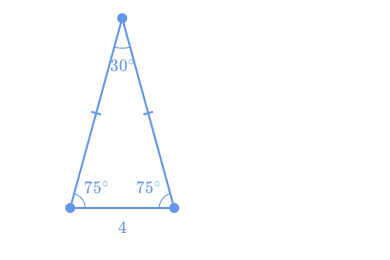
\includegraphics[scale=\shrinkfactor]{figures/8664b06c420b8bf33711310103a6963e0f2cc7f1.png}

This triangle is unique, meaning no other triangle exists \DIFdelbegin \DIFdel{that satisfies these conditions}\DIFdelend \DIFaddbegin \DIFadd{with the same shape and size}\DIFaddend .

\paragraph{Hint 3}When the side length is known between two known angles, only one triangle can be drawn.



\medskip
\noindent
\textbf{Tags:} {\footnotesize Constructing triangles, CC.7.G.A.2}\\
\textbf{Version:} \DIFdelbegin \DIFdel{e08d4e9d.. 2013-10-20
}\DIFdelend \DIFaddbegin \DIFadd{4a925246.. 2013-10-21
}\DIFaddend \smallskip\hrule





\section{\href{https://www.khanacademy.org/devadmin/content/items/x18341f6f8d24d96e}{x18341f6f8d24d96e}}

\noindent
**How many triangles can be drawn with side lengths $9$, $12$ and $15$?**



\paragraph{Ans} 

None

\fbox{ Only one

}

 More than one



\paragraph{Hint 1}A triangle is a plane figure with \DIFdelbegin \DIFdel{$3$ }\DIFdelend \DIFaddbegin \DIFadd{three }\DIFaddend straight sides and \DIFdelbegin \DIFdel{$3$ }\DIFdelend \DIFaddbegin \DIFadd{three }\DIFaddend angles. Can we satisfy the definition given the conditions? Let's try to draw a triangle given the conditions.

\paragraph{Hint 2}In general, \DIFdelbegin \DIFdel{the longest }\DIFdelend \DIFaddbegin \DIFadd{any }\DIFaddend side of a triangle \DIFdelbegin \DIFdel{must be }\DIFdelend \DIFaddbegin \DIFadd{is always }\DIFaddend shorter than the sum of the \DIFdelbegin \DIFdel{two other sides. Because $\blue{9}+\blue{12} =\blue{21}$, the two sides$\blue{9}$ and $\blue{12}$ meet to form $2$ angles with the side of length $\blue{15}$. Thus, we }\DIFdelend \DIFaddbegin \DIFadd{other two sides:
}

\begin{align*}\DIFadd{\phantom{over}\blue{15} }&\DIFadd{<\blue{9}+\blue{12} }\\\DIFadd{\phantom{over}\blue{12}}&\DIFadd{<
 \blue{9}+\blue{15} }\\\DIFadd{\phantom{over}\blue{9}}&\DIFadd{<
 \blue{12}+\blue{15} }\\\end{align*}

\DIFadd{We }\DIFaddend can create a triangle \DIFdelbegin \DIFdel{whose sides to satisfy the given conditions}\DIFdelend \DIFaddbegin \DIFadd{with a unique size and shape}\DIFaddend .


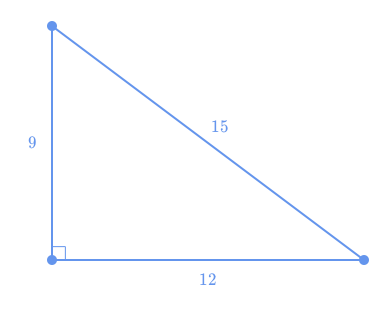
\includegraphics[scale=\shrinkfactor]{figures/9e3335e4646b2e59f3ceb8860cd9099de97f22b0.png}

\paragraph{Hint 3}Given the conditions, only one triangle can be drawn.



\medskip
\noindent
\textbf{Tags:} {\footnotesize Constructing triangles, CC.7.G.A.2}\\
\textbf{Version:} \DIFdelbegin \DIFdel{d17e39e1.. 2013-10-20
}\DIFdelend \DIFaddbegin \DIFadd{49159f6f.. 2013-10-21
}\DIFaddend \smallskip\hrule





\section{\href{https://www.khanacademy.org/devadmin/content/items/x1afa3df30210708e}{x1afa3df30210708e}}

\noindent
**Draw a \DIFaddbegin \DIFadd{right }\DIFaddend triangle with side lengths $5a$,  $12a$ and $13a$, where $a$ is any positive number.**

\DIFdelbegin \DIFdel{**Given these criteria, is the triangle unique }\DIFdelend \DIFaddbegin \DIFadd{**Is there a unique triangle that satisfies the given conditions}\DIFaddend ?**  
[[? interactive-graph 1]]

\paragraph{Ans} 

Yes

\fbox{ No

}

 

\paragraph{Hint 1}Let�s start by choosing a value for $\pink{a}$ where \DIFdelbegin \DIFdel{$\pink{a}>0$}\DIFdelend \DIFaddbegin \DIFadd{$\pink{a}$ is any positive number}\DIFaddend , then we can draw a \DIFaddbegin \DIFadd{right }\DIFaddend triangle with side lengths $\purple5\pink{a}$, $\purple{12}\pink{a}$ and $\purple{13}\pink{a}$.

\paragraph{Hint 2}Choosing $\pink{a}=\pink{1}$, we can draw a \DIFaddbegin \DIFadd{right }\DIFaddend triangle with side lengths  $\blue{5}$, $\blue{12}$ and $\blue{13}$.
\DIFdelbegin \DIFdel{This is a right triangle. 
}\DIFdelend 


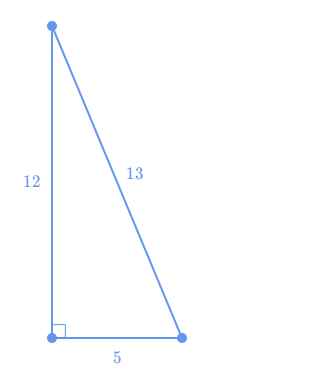
\includegraphics[scale=\shrinkfactor]{figures/6d298ed14c507f692b6d88792d963d7008b9847a.png}

\paragraph{Hint 3}Choosing $\pink{a}=\pink{0.5}$, we can draw a right triangle with side lengths $\blue{2.5}$, $\blue{6}$ and $\blue{6.5}$.   

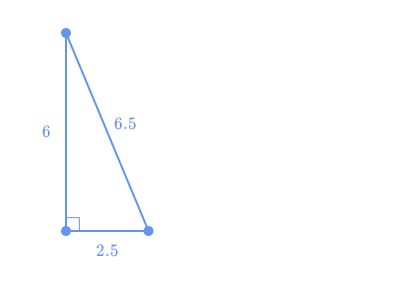
\includegraphics[scale=\shrinkfactor]{figures/463955e595c31361c49d853aea12289b0f5f7779.png} 


\paragraph{Hint 4}The triangle is not unique. We can let $\pink{a}$ be any \DIFdelbegin \DIFdel{nonzero }\DIFdelend positive number and draw many triangles with the same shape but different sizes.


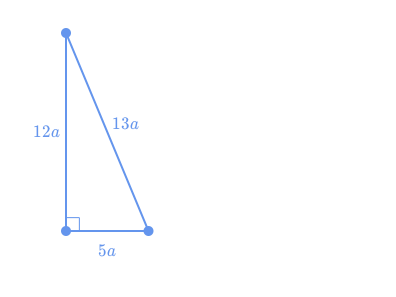
\includegraphics[scale=\shrinkfactor]{figures/28bab6f73b266fa0cb6392a48f06caca532f0cd2.png}



\medskip
\noindent
\textbf{Tags:} {\footnotesize Constructing triangles, CC.7.G.A.2}\\
\textbf{Version:} \DIFdelbegin \DIFdel{e7274d62.. 2013-10-20
}\DIFdelend \DIFaddbegin \DIFadd{f00b6980.. 2013-10-21
}\DIFaddend \smallskip\hrule





\section{\href{https://www.khanacademy.org/devadmin/content/items/x1c875467bbf94500}{x1c875467bbf94500}}

\noindent
**Draw a triangle with side length $4$ between two $70^\circ$ angles.** 

\DIFdelbegin \DIFdel{**Given these criteria is the triangle unique }\DIFdelend \DIFaddbegin \DIFadd{**Is there a unique triangle that satisfies the given conditions}\DIFaddend ?**
[[? interactive-graph 1]]

\paragraph{Ans} 

\fbox{ Yes

}

 No



\paragraph{Hint 1}Let�s start by drawing the side whose length  is $\blue{4}$.

\paragraph{Hint 2}From the side $\blue4$, let�s draw \DIFdelbegin \DIFdel{$2$ }\DIFdelend \DIFaddbegin \DIFadd{two }\DIFaddend $\blue{70^\circ}$ angles. Since we have \DIFdelbegin \DIFdel{$2$ }\DIFdelend \DIFaddbegin \DIFadd{two }\DIFaddend equal angles, we have an isosceles triangle. An isosceles triangle has at least \DIFdelbegin \DIFdel{$2$ }\DIFdelend \DIFaddbegin \DIFadd{two }\DIFaddend sides equal in length. 

Since we have \DIFdelbegin \DIFdel{$2$ }\DIFdelend \DIFaddbegin \DIFadd{two }\DIFaddend $\blue{70^\circ}$ angles, the third angle must be $\green{40^\circ}$. The sum of \DIFdelbegin \DIFdel{$3$ }\DIFdelend \DIFaddbegin \DIFadd{three }\DIFaddend angles in a triangle will always be $\pink{180^\circ}$.

\paragraph{Hint 3}We know the measure of \DIFdelbegin \DIFdel{$2$ }\DIFdelend \DIFaddbegin \DIFadd{two }\DIFaddend angles and the length of the side between the angles, so we can draw only \DIFdelbegin \DIFdel{$1$ }\DIFdelend \DIFaddbegin \DIFadd{one }\DIFaddend triangle.

\paragraph{Hint 4}The triangle is unique.


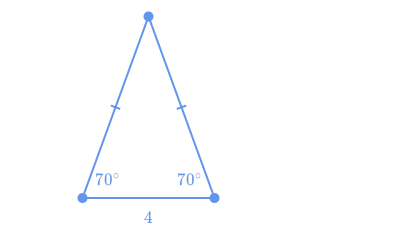
\includegraphics[scale=\shrinkfactor]{figures/42e1efd00be59b64d19c796b09c66213066bd2fa.png}



\medskip
\noindent
\textbf{Tags:} {\footnotesize Constructing triangles, CC.7.G.A.2}\\
\textbf{Version:} \DIFdelbegin \DIFdel{dd847b40.. 2013-10-20
}\DIFdelend \DIFaddbegin \DIFadd{7647d185.. 2013-10-21
}\DIFaddend \smallskip\hrule





\section{\href{https://www.khanacademy.org/devadmin/content/items/x1da87b180aca0e3d}{x1da87b180aca0e3d}}

\noindent
**How many triangles can be drawn which have side lengths of $5$ and $10$?**

\paragraph{Ans} 

None

Only one

\fbox{ More than one

}

 

\paragraph{Hint 1}We do not know the length of the third side so we are free to choose any length. Thus, we cannot create a unique triangle with only two side lengths.

\paragraph{Hint 2}We can  draw many triangles with side lengths $\blue5$ and $\blue{10}$.


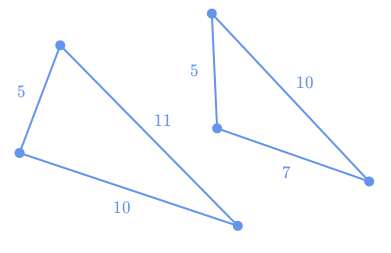
\includegraphics[scale=\shrinkfactor]{figures/fe9bb66c73daee381242a48159a578e8b78ac0fb.png}

\paragraph{Hint 3}If we only know \DIFdelbegin \DIFdel{$2$ }\DIFdelend \DIFaddbegin \DIFadd{two }\DIFaddend side lengths, more than one triangle can be drawn.



\medskip
\noindent
\textbf{Tags:} {\footnotesize Constructing triangles, CC.7.G.A.2}\\
\textbf{Version:} \DIFdelbegin \DIFdel{cd0bdb35.. 2013-10-20
}\DIFdelend \DIFaddbegin \DIFadd{d74ae956.. 2013-10-21
}\DIFaddend \smallskip\hrule





\section{\href{https://www.khanacademy.org/devadmin/content/items/x25470998d7b41ee4}{x25470998d7b41ee4}}

\noindent
**How many triangles can be drawn which have two $45^\circ$ angles and two sides of length $2$?**

\paragraph{Ans} 

None

\fbox{ Only one

}

 More than one



\paragraph{Hint 1}A triangle is a plane figure with \DIFdelbegin \DIFdel{$3$ }\DIFdelend \DIFaddbegin \DIFadd{three }\DIFaddend straight sides and \DIFdelbegin \DIFdel{$3$ }\DIFdelend \DIFaddbegin \DIFadd{three }\DIFaddend angles. The \DIFdelbegin \DIFdel{$3$ }\DIFdelend \DIFaddbegin \DIFadd{three }\DIFaddend angles always add up to $\pink{180^\circ}$. 

\DIFdelbegin \DIFdel{We }\DIFdelend \DIFaddbegin \DIFadd{Since we }\DIFaddend have two $\blue{45^\circ}$ angles\DIFdelbegin \DIFdel{. The third angle $x$ }\DIFdelend \DIFaddbegin \DIFadd{, the third angle }\DIFaddend is $\blue{90^\circ}$: 

\DIFdelbegin \begin{eqnarray*}\DIFdel{ 
\pink{180^\circ}}&\DIFdel{= \blue{45^\circ}+\blue{45^\circ} + x }\\ \DIFdel{\pink{180^\circ}}&\DIFdel{= \blue{90^\circ} + x }\\
\DIFdel{x }&\DIFdel{= \pink{180^\circ}-\blue{90^\circ} }\\
\DIFdel{x }&\DIFdel{= \blue{90^\circ} }\end{eqnarray*}
\DIFdelend \DIFaddbegin \begin{align*}\DIFadd{\
 }&\DIFadd{= \pink{180^\circ}-2\cdot\blue{45^\circ} }\\
 &\DIFadd{= \blue{90^\circ} }\end{align*}
\DIFaddend 

\DIFdelbegin \DIFdel{The third angle $x$ is $\blue{90^\circ}$ so let}\DIFdelend \DIFaddbegin \DIFadd{Let}\DIFaddend 's draw a right triangle. 

\paragraph{Hint 2}We can draw a right triangle and make two of its sides of length $\blue{2}$. The sides with length $\blue{2}$ \DIFdelbegin \DIFdel{are in }\DIFdelend \DIFaddbegin \DIFadd{must be }\DIFaddend between the $\blue{45^\circ}$ and $\blue{90^\circ}$ angles.


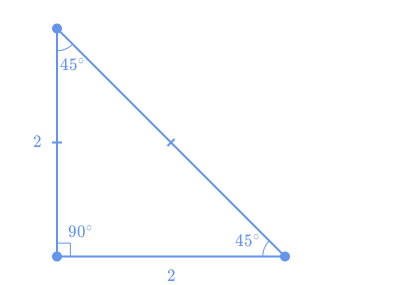
\includegraphics[scale=\shrinkfactor]{figures/50ab52075216ec1ebe030aa80de8615558c71846.png}

This triangle is unique, meaning no other triangle exists with exactly the same shape and size.

\paragraph{Hint 3}Given the conditions, only one triangle can be drawn.



\medskip
\noindent
\textbf{Tags:} {\footnotesize Constructing triangles, CC.7.G.A.2}\\
\textbf{Version:} \DIFdelbegin \DIFdel{5c0563e0.. 2013-10-20
}\DIFdelend \DIFaddbegin \DIFadd{2c26d431.. 2013-10-21
}\DIFaddend \smallskip\hrule





\section{\href{https://www.khanacademy.org/devadmin/content/items/x2bce84b97313fd2b}{x2bce84b97313fd2b}}

\noindent
**Draw a triangle \DIFdelbegin \DIFdel{where the }\DIFdelend \DIFaddbegin \DIFadd{with two angles $31^\circ$ and $90^\circ$ where }\DIFaddend side length $3$ is \DIFdelbegin \DIFdel{not between }\DIFdelend \DIFaddbegin \DIFadd{*not* between the }\DIFaddend two angles $31^\circ$ and $90^\circ$.**

\DIFdelbegin \DIFdel{**Given these criteria is the triangle unique }\DIFdelend \DIFaddbegin \DIFadd{**Is there a unique triangle that satisfies the given conditions}\DIFaddend ?**
[[? interactive-graph 1]]

\paragraph{Ans} 

\fbox{ Yes

}

 No



\paragraph{Hint 1}Let�s start by drawing a right angle which is $\blue{90^\circ}$. 

Then, let's draw the side of length $\blue3$ next to the right angle, so our base is length $\blue3$.

\paragraph{Hint 2}The length of $\blue3$ is $\red{\text{not}}$ between \DIFdelbegin \DIFdel{$2$ }\DIFdelend \DIFaddbegin \DIFadd{two }\DIFaddend angles $\blue{31^\circ}$ and $\blue{90^\circ}$. 

Since we drew the side of length $\blue3$ next to the right angle, the $\blue{31^\circ}$ angle must be *opposite* the side of length $\blue3$ .

\paragraph{Hint 3}We know the measure of \DIFdelbegin \DIFdel{$2$ }\DIFdelend \DIFaddbegin \DIFadd{two }\DIFaddend angles and the length of \DIFdelbegin \DIFdel{$1$ }\DIFdelend \DIFaddbegin \DIFadd{one }\DIFaddend side not between the angles, so we can draw only \DIFdelbegin \DIFdel{$1$ }\DIFdelend \DIFaddbegin \DIFadd{one }\DIFaddend triangle.

\paragraph{Hint 4}The triangle is unique.


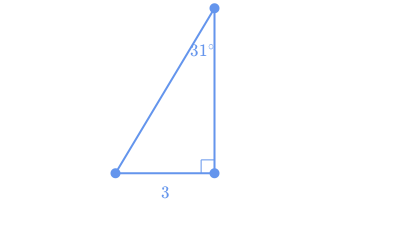
\includegraphics[scale=\shrinkfactor]{figures/48773248b446b970cdf6c2fa7664c3fa8890378a.png}



\medskip
\noindent
\textbf{Tags:} {\footnotesize Constructing triangles, CC.7.G.A.2}\\
\textbf{Version:} \DIFdelbegin \DIFdel{1215aaf1.. 2013-10-17
}\DIFdelend \DIFaddbegin \DIFadd{4c8a5b03.. 2013-10-21
}\DIFaddend \smallskip\hrule





\section{\href{https://www.khanacademy.org/devadmin/content/items/x31c216ff88dad8e7}{x31c216ff88dad8e7}}

\noindent
**How many triangles can we draw with side lengths $4$, $4$ and $7$?**

\paragraph{Ans} 

None

\fbox{ Only one

}

 More than one



\paragraph{Hint 1}A triangle is a plane figure with \DIFdelbegin \DIFdel{$3$ }\DIFdelend \DIFaddbegin \DIFadd{three }\DIFaddend straight sides and \DIFdelbegin \DIFdel{$3$ }\DIFdelend \DIFaddbegin \DIFadd{three }\DIFaddend angles. Can we satisfy the definition given the conditions? Let's try to draw a triangle given the conditions.

\paragraph{Hint 2}In general, \DIFdelbegin \DIFdel{the longest }\DIFdelend \DIFaddbegin \DIFadd{any }\DIFaddend side of a triangle \DIFdelbegin \DIFdel{must be }\DIFdelend \DIFaddbegin \DIFadd{is always }\DIFaddend shorter than the sum of the \DIFdelbegin \DIFdel{two other sides. Because $\blue{4}+\blue{4} =\blue{8}$, the two sides$\blue{4}$ and $\blue{4}$ meet to form $2$ angles with the side of length $\blue{7}$. }\DIFdelend \DIFaddbegin \DIFadd{other two sides:
}

\begin{align*}\DIFadd{\phantom{over}\blue{7} }&\DIFadd{<\blue{4}+\blue{4} }\\\DIFadd{\phantom{over}\blue{4}}&\DIFadd{<
 \blue{7}+\blue{4}  }\\\end{align*}

\DIFaddend We can create \DIFdelbegin \DIFdel{$3$ angles with the $3$ sides to satisfy the definition of a triangle }\DIFdelend \DIFaddbegin \DIFadd{a triangle with a unique size and shape}\DIFaddend .


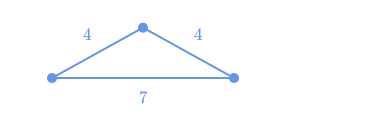
\includegraphics[scale=\shrinkfactor]{figures/a5961a517a4e6e5e6def530e3948dc049dbfad9a.png}

\paragraph{Hint 3}Given the conditions, only one triangle can be drawn.



\medskip
\noindent
\textbf{Tags:} {\footnotesize Constructing triangles, CC.7.G.A.2}\\
\textbf{Version:} \DIFdelbegin \DIFdel{33683619..2013-10-20
}\DIFdelend \DIFaddbegin \DIFadd{7bc13eed.. 2013-10-21
}\DIFaddend \smallskip\hrule





\section{\href{https://www.khanacademy.org/devadmin/content/items/x38cc51ab93842600}{x38cc51ab93842600}}

\noindent
**How many triangles can be drawn with side lengths $1$, $1$ and \DIFdelbegin \DIFdel{$2$}\DIFdelend \DIFaddbegin \DIFadd{$2.5$}\DIFaddend ?**

\paragraph{Ans} 

\fbox{ None

}

 Only one

More than one



\paragraph{Hint 1}A triangle is a plane figure with \DIFdelbegin \DIFdel{$3$ }\DIFdelend \DIFaddbegin \DIFadd{three }\DIFaddend straight sides and \DIFdelbegin \DIFdel{$3$ }\DIFdelend \DIFaddbegin \DIFadd{three }\DIFaddend angles. Can we satisfy the definition given the conditions? Let's try to draw a triangle given the conditions.

\paragraph{Hint 2}In general, \DIFdelbegin \DIFdel{the longest }\DIFdelend \DIFaddbegin \DIFadd{any }\DIFaddend side of a triangle \DIFdelbegin \DIFdel{must be }\DIFdelend \DIFaddbegin \DIFadd{is always }\DIFaddend shorter than the sum of the \DIFdelbegin \DIFdel{two other }\DIFdelend \DIFaddbegin \DIFadd{other two }\DIFaddend sides. Because \DIFdelbegin \DIFdel{$\blue{1}+\blue{1} =\blue{2}$}\DIFdelend \DIFaddbegin \DIFadd{$\blue{2.5} >\blue{1}+\blue{1}$}\DIFaddend , the two \DIFdelbegin \DIFdel{side lengths }\DIFdelend \DIFaddbegin \DIFadd{sides }\DIFaddend $\blue{1}$ and $\blue{1}$ cannot meet to form a third angle \DIFdelbegin \DIFdel{. }\DIFdelend \DIFaddbegin \DIFadd{over the third side $\blue{2.5}$. 
}


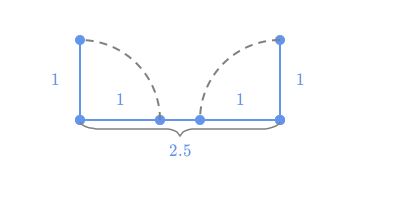
\includegraphics[scale=\shrinkfactor]{figures/cb4884edd39739116b62d131aa206b66f99db2cb.png}

\DIFaddend We cannot create \DIFdelbegin \DIFdel{$3$ }\DIFdelend \DIFaddbegin \DIFadd{three }\DIFaddend angles to satisfy the definition of a triangle.

\DIFdelbegin 
\DIFdelend \paragraph{Hint 3}Given the conditions, no triangles can be drawn.



\medskip
\noindent
\textbf{Tags:} {\footnotesize Constructing triangles, CC.7.G.A.2}\\
\textbf{Version:} \DIFdelbegin \DIFdel{aeb719e4.. 2013-10-18
}\DIFdelend \DIFaddbegin \DIFadd{05f2acc5.. 2013-10-21
}\DIFaddend \smallskip\hrule





\section{\href{https://www.khanacademy.org/devadmin/content/items/x4c335bfbee0cba92}{x4c335bfbee0cba92}}

\noindent
**Draw a right triangle with at least \DIFdelbegin \DIFdel{$2$ }\DIFdelend \DIFaddbegin \DIFadd{two }\DIFaddend sides of equal length.** 

\DIFdelbegin \DIFdel{**Given these criteria is the triangle unique }\DIFdelend \DIFaddbegin \DIFadd{**Is there a unique triangle that satisfies the given conditions}\DIFaddend ?**
[[? interactive-graph 1]]

\paragraph{Ans} 

Yes

\fbox{ No

}

 

\paragraph{Hint 1}Let�s start by drawing. A right triangle has one $\blue{90 ^\circ}$ angle. 

A triangle with at least \DIFdelbegin \DIFdel{$2$ }\DIFdelend \DIFaddbegin \DIFadd{two }\DIFaddend equal side lengths is called an isosceles triangle. We do not know the side lengths.

\paragraph{Hint 2}We can draw many right triangles with \DIFdelbegin \DIFdel{$2$ }\DIFdelend \DIFaddbegin \DIFadd{two }\DIFaddend sides of  equal length.  

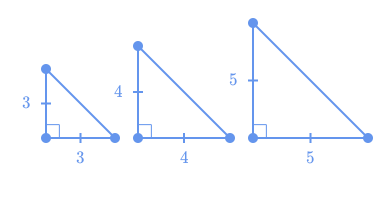
\includegraphics[scale=\shrinkfactor]{figures/d8b2dd5b2d43266692ba3d2c35cf5638f2f3c05c.png}

\paragraph{Hint 3}The triangle is not unique.



\medskip
\noindent
\textbf{Tags:} {\footnotesize Constructing triangles, CC.7.G.A.2}\\
\textbf{Version:} \DIFdelbegin \DIFdel{5f71c91d.. 2013-10-20
}\DIFdelend \DIFaddbegin \DIFadd{381a8a90.. 2013-10-21
}\DIFaddend \smallskip\hrule





\section{\href{https://www.khanacademy.org/devadmin/content/items/x531e157ba7c498eb}{x531e157ba7c498eb}}

\noindent
**How many triangles can be drawn where the measures of all \DIFdelbegin \DIFdel{$3$ }\DIFdelend \DIFaddbegin \DIFadd{three }\DIFaddend angles are the same?**

\paragraph{Ans} 

None

Only one

\fbox{ More than one

}

 

\paragraph{Hint 1}A triangle is a plane figure with \DIFdelbegin \DIFdel{$3$ }\DIFdelend \DIFaddbegin \DIFadd{three }\DIFaddend straight sides and \DIFdelbegin \DIFdel{$3$ }\DIFdelend \DIFaddbegin \DIFadd{three }\DIFaddend angles. What triangle or triangles would satisfy the conditions? 

Let's try to draw a triangle where the measures of all \DIFdelbegin \DIFdel{$3$ }\DIFdelend \DIFaddbegin \DIFadd{three }\DIFaddend angles is the same. 

\paragraph{Hint 2}The \DIFdelbegin \DIFdel{$3$ }\DIFdelend \DIFaddbegin \DIFadd{three }\DIFaddend angle measures in a triangle must sum to \DIFdelbegin \DIFdel{$180^\circ$}\DIFdelend \DIFaddbegin \DIFadd{$\pink{180^\circ}$}\DIFaddend . Because we know the measure of all \DIFdelbegin \DIFdel{$3$ }\DIFdelend \DIFaddbegin \DIFadd{three }\DIFaddend angles must be the same, we know all \DIFdelbegin \DIFdel{$3$ }\DIFdelend \DIFaddbegin \DIFadd{three }\DIFaddend angles have measure \DIFdelbegin \DIFdel{$\dfrac{180^\circ}{3}=\blue{60^\circ}$}\DIFdelend \DIFaddbegin \DIFadd{$\dfrac{\pink{180^\circ}}{3}=\blue{60^\circ}$}\DIFaddend . 


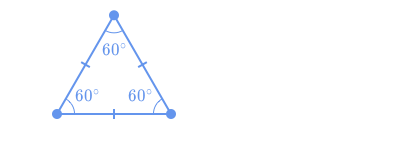
\includegraphics[scale=\shrinkfactor]{figures/9bbd0fa30a5ae16d50c816c4a8c4cfc44a68146c.png}

This is an equilateral triangle.


\paragraph{Hint 3}Is this triangle unique or do other equilateral triangles exist with a different size?

We can draw many equilateral triangles with the same shape but different sizes.


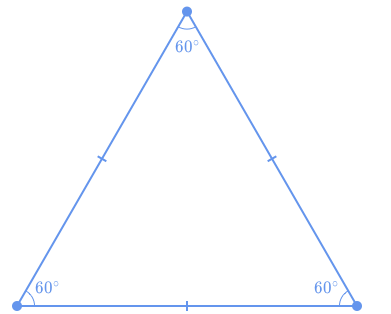
\includegraphics[scale=\shrinkfactor]{figures/3e0462daa95058cdd7264a43f9c163723c418fd6.png}

\paragraph{Hint 4}More than one triangle can be drawn with all \DIFdelbegin \DIFdel{$3$ }\DIFdelend \DIFaddbegin \DIFadd{three }\DIFaddend angles measures equal.



\medskip
\noindent
\textbf{Tags:} {\footnotesize Constructing triangles, CC.7.G.A.2}\\
\textbf{Version:} \DIFdelbegin \DIFdel{47228a28.. 2013-10-20
}\DIFdelend \DIFaddbegin \DIFadd{1ab79063.. 2013-10-21
}\DIFaddend \smallskip\hrule





\section{\href{https://www.khanacademy.org/devadmin/content/items/x572fecbc70b353aa}{x572fecbc70b353aa}}

\noindent
**Draw a right triangle that is also an isosceles triangle and has two sides of length $3$.** 

\DIFdelbegin \DIFdel{**Given these criteria is the triangle unique }\DIFdelend \DIFaddbegin \DIFadd{**Is there a unique triangle that satisfies the given conditions}\DIFaddend ?**   
[[? interactive-graph 1]]

\paragraph{Ans} 

\fbox{ Yes

}

 No



\paragraph{Hint 1}Let�s start by drawing. A right triangle has one $\blue{90^\circ}$ angle. 

An isosceles triangle has at least \DIFdelbegin \DIFdel{$2$ }\DIFdelend \DIFaddbegin \DIFadd{two }\DIFaddend side lengths equal. We are given \DIFdelbegin \DIFdel{$2$ }\DIFdelend \DIFaddbegin \DIFadd{two }\DIFaddend side lengths both equal to $\blue3$. 

\paragraph{Hint 2}Let's draw \DIFdelbegin \DIFdel{$1$ }\DIFdelend \DIFaddbegin \DIFadd{one }\DIFaddend side length $\blue{3}$ as the height vertically (up and down) from the $\blue{90 ^\circ}$ angle. Let's draw the other side length $\blue{3}$ as the base horizontally (left and right) from the $\blue{90^\circ}$ angle. 

\paragraph{Hint 3}Since we are given the measures of \DIFdelbegin \DIFdel{$2$ }\DIFdelend \DIFaddbegin \DIFadd{two }\DIFaddend sides and the angle between them, we can draw only \DIFdelbegin \DIFdel{$1$ }\DIFdelend \DIFaddbegin \DIFadd{one }\DIFaddend triangle.

\paragraph{Hint 4}The triangle is unique.

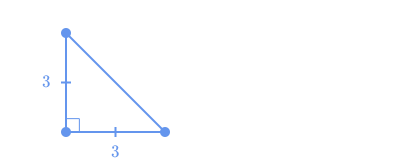
\includegraphics[scale=\shrinkfactor]{figures/29740936508e0ec4c2d3167e2aec0f3372ce78bf.png}



\medskip
\noindent
\textbf{Tags:} {\footnotesize Constructing triangles, CC.7.G.A.2}\\
\textbf{Version:} \DIFdelbegin \DIFdel{b8c14c25.. 2013-10-20
}\DIFdelend \DIFaddbegin \DIFadd{42221dd1.. 2013-10-21
}\DIFaddend \smallskip\hrule





\section{\href{https://www.khanacademy.org/devadmin/content/items/x651844ecfaac48e9}{x651844ecfaac48e9}}

\noindent
**Draw a right triangle with two $45^\circ$ angles.**

\DIFdelbegin \DIFdel{**Given these criteria is the triangle unique }\DIFdelend \DIFaddbegin \DIFadd{**Is there a unique triangle that satisfies the given conditions}\DIFaddend ?**
[[? interactive-graph 1]]

\paragraph{Ans} 

Yes

\fbox{ No

}

 

\paragraph{Hint 1}Let�s start by drawing. A right triangle has one $\blue{90^\circ}$ angle. 

The triangle we want is an isosceles right triangle. An isosceles right triangle has two $\blue{45^\circ}$ angles.

\paragraph{Hint 2}We know the measure of all \DIFdelbegin \DIFdel{$3$ }\DIFdelend \DIFaddbegin \DIFadd{three }\DIFaddend angles but not the length of any side. Therefore, we can draw many triangles of various sizes all with a pair of $\blue{45^\circ}$ angles.


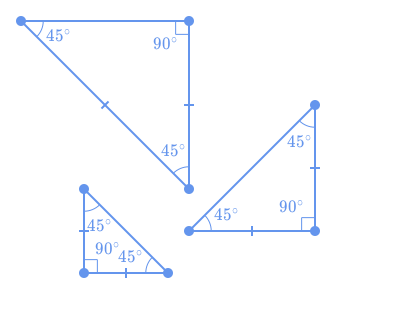
\includegraphics[scale=\shrinkfactor]{figures/91996cb5320f958d2fa0f8249c77e9d88bbb2764.png}


\paragraph{Hint 3}The triangle is not unique.




\medskip
\noindent
\textbf{Tags:} {\footnotesize Constructing triangles, CC.7.G.A.2}\\
\textbf{Version:} \DIFdelbegin \DIFdel{525a66e3.. 2013-10-20
}\DIFdelend \DIFaddbegin \DIFadd{fb842816.. 2013-10-21
}\DIFaddend \smallskip\hrule





\section{\href{https://www.khanacademy.org/devadmin/content/items/x6763ceb1ec0ceb41}{x6763ceb1ec0ceb41}}

\noindent
**How many triangles can be drawn where the lengths of all \DIFdelbegin \DIFdel{$3$ }\DIFdelend \DIFaddbegin \DIFadd{three }\DIFaddend sides are equal to $1$?**

\paragraph{Ans} 

None

\fbox{ Only one

}

 More than one



\paragraph{Hint 1}A triangle is a plane figure with \DIFdelbegin \DIFdel{$3$ }\DIFdelend \DIFaddbegin \DIFadd{three }\DIFaddend straight sides and \DIFdelbegin \DIFdel{$3$ }\DIFdelend \DIFaddbegin \DIFadd{three }\DIFaddend angles. Is there a triangle or triangles that satisfy the conditions? Let's try to draw a triangle with all side lengths equal to \DIFdelbegin \DIFdel{$1$}\DIFdelend \DIFaddbegin \DIFadd{$\blue1$}\DIFaddend .

\paragraph{Hint 2}The result is an equilateral triangle with equal side lengths and equal angles measures:


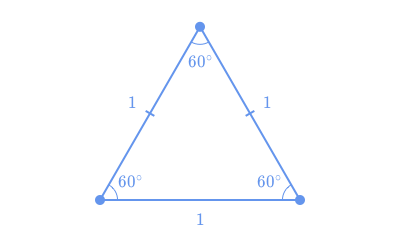
\includegraphics[scale=\shrinkfactor]{figures/b0e7ebe35f997eac2f27bbad47f0033422d118b3.png}

This triangle is unique, meaning no other triangle exists that has all sides equal to \DIFdelbegin \DIFdel{$1$}\DIFdelend \DIFaddbegin \DIFadd{$\blue1$}\DIFaddend .

\paragraph{Hint 3}In general, if the lengths of all \DIFdelbegin \DIFdel{$3$ }\DIFdelend \DIFaddbegin \DIFadd{three }\DIFaddend sides are known, only one triangle can be drawn.



\medskip
\noindent
\textbf{Tags:} {\footnotesize Constructing triangles, CC.7.G.A.2}\\
\textbf{Version:} \DIFdelbegin \DIFdel{ca634aaf.. 2013-10-20
}\DIFdelend \DIFaddbegin \DIFadd{e412934c.. 2013-10-21
}\DIFaddend \smallskip\hrule





\section{\href{https://www.khanacademy.org/devadmin/content/items/x67ee6010588311f2}{x67ee6010588311f2}}

\noindent
**How many triangles can be drawn with side lengths $4$, $6$ and \DIFdelbegin \DIFdel{$10$}\DIFdelend \DIFaddbegin \DIFadd{$11$}\DIFaddend ?**

\paragraph{Ans} 

\fbox{ None

}

 Only one

More than one



\paragraph{Hint 1}A triangle is a plane figure with \DIFdelbegin \DIFdel{$3$ }\DIFdelend \DIFaddbegin \DIFadd{three }\DIFaddend straight sides and \DIFdelbegin \DIFdel{$3$ }\DIFdelend \DIFaddbegin \DIFadd{three }\DIFaddend angles. Can we satisfy the definition given the conditions? Let's try to draw a triangle given the conditions.

\paragraph{Hint 2}In general, \DIFdelbegin \DIFdel{the longest }\DIFdelend \DIFaddbegin \DIFadd{any }\DIFaddend side of a triangle \DIFdelbegin \DIFdel{must be }\DIFdelend \DIFaddbegin \DIFadd{is always }\DIFaddend shorter than the sum of the \DIFdelbegin \DIFdel{two other }\DIFdelend \DIFaddbegin \DIFadd{other two }\DIFaddend sides. Because \DIFdelbegin \DIFdel{$\blue{4}+\blue{6} =\blue{10}$}\DIFdelend \DIFaddbegin \DIFadd{$\blue{11} >\blue{6}+\blue{4}$}\DIFaddend , the two sides \DIFdelbegin \DIFdel{$\blue{4}$ and }\DIFdelend $\blue{6}$ \DIFaddbegin \DIFadd{and $\blue{4}$ }\DIFaddend cannot meet to form a third angle \DIFdelbegin \DIFdel{. }\DIFdelend \DIFaddbegin \DIFadd{over the third side $\blue{11}$. 
}


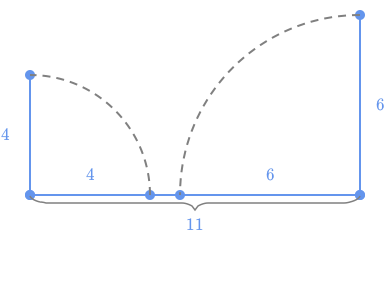
\includegraphics[scale=\shrinkfactor]{figures/6b60caa69910861ed0aa6e21b79d5cde304168b3.png}

\DIFaddend We cannot create \DIFdelbegin \DIFdel{$3$ }\DIFdelend \DIFaddbegin \DIFadd{three }\DIFaddend angles to satisfy the definition of a triangle.

\DIFdelbegin 
\DIFdelend \paragraph{Hint 3}Given the conditions, no triangles can be drawn.



\medskip
\noindent
\textbf{Tags:} {\footnotesize Constructing triangles, CC.7.G.A.2}\\
\textbf{Version:} \DIFdelbegin \DIFdel{9421cd19.. 2013-10-18
}\DIFdelend \DIFaddbegin \DIFadd{edcac7f5.. 2013-10-21
}\DIFaddend \smallskip\hrule





\section{\href{https://www.khanacademy.org/devadmin/content/items/x67fd10caf4f54df2}{x67fd10caf4f54df2}}

\noindent
**Draw a \DIFaddbegin \DIFadd{right }\DIFaddend triangle with side lengths $3a$,  $4a$ and $5a$, where $a$ is any positive number.**

\DIFdelbegin \DIFdel{**Given these criteria is the triangle unique }\DIFdelend \DIFaddbegin \DIFadd{**Is there a unique triangle that satisfies the given conditions}\DIFaddend ?**
[[? interactive-graph 1]]

\paragraph{Ans} 

Yes

\fbox{ No

}

 

\paragraph{Hint 1}Let�s start by choosing a value for $\pink{a}$ where \DIFdelbegin \DIFdel{$\pink{a}>0$}\DIFdelend \DIFaddbegin \DIFadd{$\pink{a}$ is any positive number}\DIFaddend , then we can draw a \DIFaddbegin \DIFadd{right }\DIFaddend triangle with side lengths $\purple3\pink{a}$, $\purple4\pink{a}$ and $\purple5\pink{a}$.

\paragraph{Hint 2}If $\pink{a}=1$, then we can draw a \DIFaddbegin \DIFadd{right }\DIFaddend triangle with side lengths $\blue3$, $\blue4$ and $\blue5$. 
\DIFdelbegin \DIFdel{This is a right triangle.
}\DIFdelend 

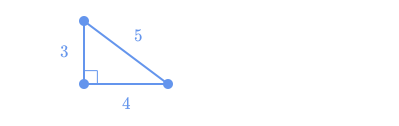
\includegraphics[scale=\shrinkfactor]{figures/b1eff2246ff6077c50f40ea6bfe55bad4b8ced80.png}

\paragraph{Hint 3}If $\pink{a}=2$, then we can draw a right triangle with side lengths $\blue6$, $\blue8$ and $\blue{10}$. 

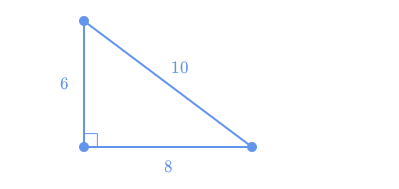
\includegraphics[scale=\shrinkfactor]{figures/ef5a8edbd9d4f5680b124ce81e7f4c78a9707ed4.png}

We can let $\pink{a}$ be any positive number and draw many triangles of same shape but different sizes.

\paragraph{Hint 4}The triangle is not unique. Multiple triangles satisfy the conditions.


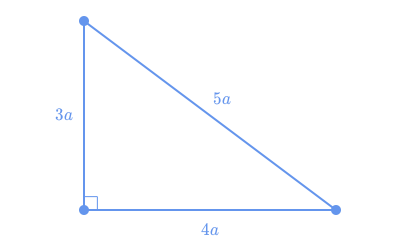
\includegraphics[scale=\shrinkfactor]{figures/946760cec54502326e2f2708bb7c84428118c9ad.png}



\medskip
\noindent
\textbf{Tags:} {\footnotesize Constructing triangles, CC.7.G.A.2}\\
\textbf{Version:} \DIFdelbegin \DIFdel{95e0a049.. 2013-10-20
}\DIFdelend \DIFaddbegin \DIFadd{0b713fdb.. 2013-10-21
}\DIFaddend \smallskip\hrule





\section{\href{https://www.khanacademy.org/devadmin/content/items/x6d7be6276bcb5815}{x6d7be6276bcb5815}}

\noindent
**Draw a right triangle with a height $4$ and base  $5$.** 

\DIFdelbegin \DIFdel{**Given these criteria is the triangle unique }\DIFdelend \DIFaddbegin \DIFadd{**Is there a unique triangle that satisfies the given conditions}\DIFaddend ?**
[[? interactive-graph 1]]

\paragraph{Ans} 

\fbox{ Yes

}

 No



\paragraph{Hint 1}Let�s start by drawing. A right triangle has a $\blue{90^\circ}$ angle. 

The height of length $\blue{4}$ is drawn vertically (up and down) from the $\blue{90^\circ}$ angle. The base of length $\blue{5}$ is drawn horizontally (left and right) from the $\blue{90^\circ}$ angle. 

\paragraph{Hint 2}Since we are given the measures of \DIFdelbegin \DIFdel{$2$ }\DIFdelend \DIFaddbegin \DIFadd{two }\DIFaddend sides and the angle between them, we can draw only \DIFdelbegin \DIFdel{$1$ }\DIFdelend \DIFaddbegin \DIFadd{one }\DIFaddend triangle.

\paragraph{Hint 3}The triangle is unique.


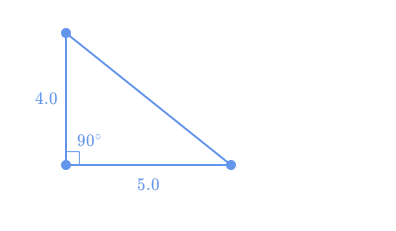
\includegraphics[scale=\shrinkfactor]{figures/21924a4df5c1451289595e8ec2c9ceae30ed7de1.png}



\medskip
\noindent
\textbf{Tags:} {\footnotesize Constructing triangles, CC.7.G.A.2}\\
\textbf{Version:} \DIFdelbegin \DIFdel{41522448.. 2013-10-20
}\DIFdelend \DIFaddbegin \DIFadd{77539544.. 2013-10-21
}\DIFaddend \smallskip\hrule





\section{\href{https://www.khanacademy.org/devadmin/content/items/x72d893d1e3229dfd}{x72d893d1e3229dfd}}

\noindent
**How many triangles can we draw with side lengths  $3$ and $4$?**

\paragraph{Ans} 

None

Only one

\fbox{ More than one

}

 

\paragraph{Hint 1}We can  draw many triangles with side lengths $\blue3$ and $\blue{4}$.


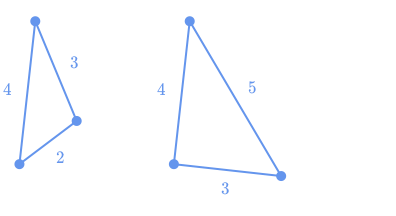
\includegraphics[scale=\shrinkfactor]{figures/2d99bebb2da26f68f4d74679d523ed8d96db3e5c.png}

\paragraph{Hint 2}Without knowing at least \DIFdelbegin \DIFdel{$1$ }\DIFdelend \DIFaddbegin \DIFadd{one }\DIFaddend angle measure, we cannot create a unique triangle with side lengths \DIFdelbegin \DIFdel{$3$ and $4$}\DIFdelend \DIFaddbegin \DIFadd{$\blue3$ and $\blue4$}\DIFaddend .

\paragraph{Hint 3}If we only know \DIFdelbegin \DIFdel{$2$ }\DIFdelend \DIFaddbegin \DIFadd{two }\DIFaddend side lengths, more than one triangle can be drawn.



\medskip
\noindent
\textbf{Tags:} {\footnotesize Constructing triangles, CC.7.G.A.2}\\
\textbf{Version:} \DIFdelbegin \DIFdel{af92749c.. 2013-10-20
}\DIFdelend \DIFaddbegin \DIFadd{7f5a7177.. 2013-10-21
}\DIFaddend \smallskip\hrule





\section{\href{https://www.khanacademy.org/devadmin/content/items/x892857b71e427c39}{x892857b71e427c39}}

\noindent
**How many triangles can be drawn with angles $60^\circ$,  $60^\circ$ and $70^\circ$?**

\paragraph{Ans} 

\fbox{ None

}

 Only one

More than one



\paragraph{Hint 1}A triangle is a plane figure with \DIFdelbegin \DIFdel{$3$ }\DIFdelend \DIFaddbegin \DIFadd{three }\DIFaddend straight sides and \DIFdelbegin \DIFdel{$3$ }\DIFdelend \DIFaddbegin \DIFadd{three }\DIFaddend angles. In a triangle, the sum of the three angle measures is $\pink{180^\circ}$.

\paragraph{Hint 2}Let's add together the angles measures $\blue{60}^\circ$,  $\blue{60}^\circ$ and $\blue{70}^\circ$:

\DIFdelbegin \begin{eqnarray*}\DIFdel{ 
\text{sum of angle measures} 
}&\DIFdel{= \blue{60^\circ} + \blue{60^\circ}+\blue{70^\circ}}\\
&\DIFdel{= 120^\circ+70^\circ}\\
&\DIFdel{= 190^\circ}\\
&\DIFdel{>\pink{180^\circ}
}\end{eqnarray*}
\DIFdelend \DIFaddbegin \begin{align*}\DIFadd{ 
\text{sum of angle measures} 
}&\DIFadd{= \blue{60^\circ} + \blue{60^\circ}+\blue{70^\circ}}\\
&\DIFadd{= 120^\circ+70^\circ}\\
&\DIFadd{= 190^\circ}\\
\end{align*}
\DIFaddend 

The sum of the \DIFdelbegin \DIFdel{$3$ }\DIFdelend \DIFaddbegin \DIFadd{three }\DIFaddend angle measures is greater than $\pink{180^\circ}$.

\paragraph{Hint 3}No triangle can be drawn that satisfies the given conditions.



\medskip
\noindent
\textbf{Tags:} {\footnotesize Constructing triangles, CC.7.G.A.2}\\
\textbf{Version:} \DIFdelbegin \DIFdel{88ce2f2f.. 2013-10-20
}\DIFdelend \DIFaddbegin \DIFadd{b659944d.. 2013-10-21
}\DIFaddend \smallskip\hrule





\DIFaddbegin \section{\href{https://www.khanacademy.org/devadmin/content/items/xb880da8414b8f195}{xb880da8414b8f195}}

\noindent
\DIFadd{**Draw an obtuse triangle with angles $45^\circ$,  $35^\circ$ and $100^\circ$.**
}

\DIFadd{**Is there a unique triangle that satisfies the given conditions?**
}[[\DIFadd{? interactive-graph 1}]]

\paragraph{{Ans}} 

\DIFadd{Yes
}

\DIFadd{\fbox{ No } }

 

\paragraph{\DIFadd{Hint 1}}\DIFadd{Let�s start by drawing. While keeping one angle constant, we can change the side lengths to create one of the other two angles.
}

\DIFadd{For example, while keeping a $\blue{45^\circ}$ angle, we can change the side lengths to create the $\blue{35^\circ}$ angle. The third angle will have measure $\blue{100^\circ}$.
}

\paragraph{\DIFadd{Hint 2}}\DIFadd{We know the measure of three angles but not the length of any side. We can draw many triangles of same shape but different sizes.
}

\paragraph{\DIFadd{Hint 3}}\DIFadd{The triangle is not unique.
}


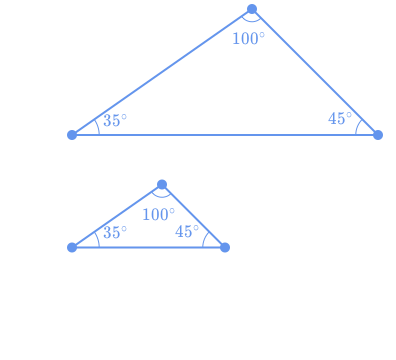
\includegraphics[scale=\shrinkfactor]{figures/c6b48cf353062cc42130d16552b68f58a6daf58e.png}



\medskip
\noindent
\textbf{\DIFadd{Tags:}} {\footnotesize \DIFadd{Constructing triangles, CC.7.G.A.2}}\\
\textbf{\DIFadd{Version:}} \DIFadd{6879cae0.. 2013-10-21
}\smallskip\hrule





\DIFaddend \section{\href{https://www.khanacademy.org/devadmin/content/items/xb9aa47b3de982d55}{xb9aa47b3de982d55}}

\noindent
**Draw an isosceles triangle with two $70^\circ$ angles.**

\DIFdelbegin \DIFdel{**Given these criteria is the triangle unique }\DIFdelend \DIFaddbegin \DIFadd{**Is there a unique triangle that satisfies the given conditions}\DIFaddend ?**
[[? interactive-graph 1]]

\paragraph{Ans} 

Yes

\fbox{ No

}

 

\paragraph{Hint 1}Let�s start by drawing an isosceles triangle with \DIFdelbegin \DIFdel{$2$ }\DIFdelend \DIFaddbegin \DIFadd{two }\DIFaddend $\blue{70^\circ}$ angles. An isosceles triangle has at least \DIFdelbegin \DIFdel{$2$ }\DIFdelend \DIFaddbegin \DIFadd{two }\DIFaddend side lengths equal and \DIFdelbegin \DIFdel{$2$ }\DIFdelend \DIFaddbegin \DIFadd{two }\DIFaddend angles equal.

\paragraph{Hint 2}We do not know the side lengths, so we can draw many triangles.

\paragraph{Hint 3}The triangle is not unique.

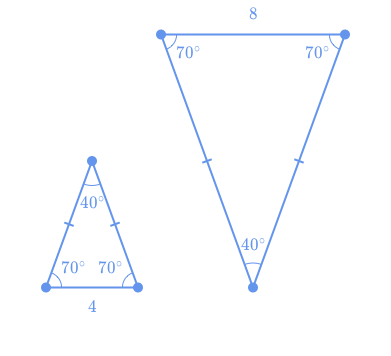
\includegraphics[scale=\shrinkfactor]{figures/afb29f0a848d89c4b6991b76cd2f1a48e594243b.png}



\medskip
\noindent
\textbf{Tags:} {\footnotesize Constructing triangles, CC.7.G.A.2}\\
\textbf{Version:} \DIFdelbegin \DIFdel{3bc9edc0.. 2013-10-18
}\DIFdelend \DIFaddbegin \DIFadd{c30a9e63.. 2013-10-21
}\DIFaddend \smallskip\hrule





\section{\href{https://www.khanacademy.org/devadmin/content/items/xbd061a8700fced6c}{xbd061a8700fced6c}}

\noindent
**How many right triangles can be drawn with angles $40^\circ$ and  $60^\circ$?**

\paragraph{Ans} 

\fbox{ None

}

 Only one

More than one



\paragraph{Hint 1}A triangle is a plane figure with \DIFdelbegin \DIFdel{$3$ }\DIFdelend \DIFaddbegin \DIFadd{three }\DIFaddend straight sides and \DIFdelbegin \DIFdel{$3$ }\DIFdelend \DIFaddbegin \DIFadd{three }\DIFaddend angles. In a triangle, the sum of the three angle measures is $\pink{180^\circ}$.

A right triangle has a $\blue{90}^\circ$  angle.

\paragraph{Hint 2}Let's add together the angle measures $\blue{40}^\circ$,  $\blue{60}^\circ$ and $\blue{90}^\circ$:

\DIFdelbegin \begin{eqnarray*}\DIFdel{
\text{sum of angle measures} 
 }&\DIFdel{=  \blue{40^\circ}+\blue{60^\circ}+\blue{90^\circ}}\\
&\DIFdel{= 190^\circ}\\&\DIFdel{>\pink{180^\circ}}\end{eqnarray*}
\DIFdelend \DIFaddbegin \begin{align*}\DIFadd{
\text{sum of angle measures} 
 }&\DIFadd{=  \blue{40^\circ}+\blue{60^\circ}+\blue{90^\circ}}\\
&\DIFadd{= 190^\circ}\end{align*}
\DIFaddend 

The sum of the \DIFdelbegin \DIFdel{$3$ }\DIFdelend \DIFaddbegin \DIFadd{three }\DIFaddend angles is greater than $\pink{180^\circ}$.

\paragraph{Hint 3}No triangle can be drawn that satisfies the given conditions.



\medskip
\noindent
\textbf{Tags:} {\footnotesize Constructing triangles, CC.7.G.A.2}\\
\textbf{Version:} \DIFdelbegin \DIFdel{69a54880.. 2013-10-20
}\DIFdelend \DIFaddbegin \DIFadd{24dc4864.. 2013-10-21
}\DIFaddend \smallskip\hrule





\section{\href{https://www.khanacademy.org/devadmin/content/items/xc001c788d01d9e5f}{xc001c788d01d9e5f}}

\noindent
**Draw a triangle \DIFaddbegin \DIFadd{with two angles $58^\circ$ and $90^\circ$ }\DIFaddend where side length $4$ is \DIFdelbegin \DIFdel{not between }\DIFdelend \DIFaddbegin \DIFadd{*not* between the }\DIFaddend two angles $58^\circ$ and $90^\circ$.**

\DIFdelbegin \DIFdel{**Given these criteria is the triangle unique }\DIFdelend \DIFaddbegin \DIFadd{**Is there a unique triangle that satisfies the given conditions}\DIFaddend ?**
[[? interactive-graph 1]]

\paragraph{Ans} 

\fbox{ Yes

}

 No



\paragraph{Hint 1}Let�s start by drawing a right angle which is $\blue{90^\circ}$. 

Then, let's draw the side of length $\blue4$ next to the right angle, so our base has a length of $\blue4$.

\paragraph{Hint 2}The side of length $\blue4$ is $\red{\text{not}}$ between \DIFdelbegin \DIFdel{$2$ }\DIFdelend \DIFaddbegin \DIFadd{two }\DIFaddend angles $\blue{58^\circ}$ and $\blue{90^\circ}$. 

Since we drew the side of length $\blue4$ next to the right angle, the $\blue{58^\circ}$ angle must be *opposite* the side of length $\blue4$ .

\paragraph{Hint 3}We know the measure of \DIFdelbegin \DIFdel{$2$ }\DIFdelend \DIFaddbegin \DIFadd{two }\DIFaddend angles and the length of \DIFdelbegin \DIFdel{$1$ }\DIFdelend \DIFaddbegin \DIFadd{one }\DIFaddend side not between the angles, so we can draw only \DIFdelbegin \DIFdel{$1$ }\DIFdelend \DIFaddbegin \DIFadd{one }\DIFaddend triangle.

\paragraph{Hint 4}The triangle is unique.


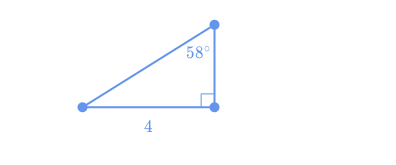
\includegraphics[scale=\shrinkfactor]{figures/0ddd88656709215709e4a46913277db7929349d4.png}



\medskip
\noindent
\textbf{Tags:} {\footnotesize Constructing triangles, CC.7.G.A.2}\\
\textbf{Version:} \DIFdelbegin \DIFdel{9534c031.. 2013-10-17
}\DIFdelend \DIFaddbegin \DIFadd{c15babbe.. 2013-10-21
}\DIFaddend \smallskip\hrule





\section{\href{https://www.khanacademy.org/devadmin/content/items/xc256611ab7d92e83}{xc256611ab7d92e83}}

\noindent
**Draw a triangle with side length $5$ between two $58^\circ$ angles.** 

\DIFdelbegin \DIFdel{**Given these criteria is the triangle unique }\DIFdelend \DIFaddbegin \DIFadd{**Is there a unique triangle that satisfies the given conditions}\DIFaddend ?**
[[? interactive-graph 1]]

\paragraph{Ans} 

\fbox{ Yes

}

 No



\paragraph{Hint 1}Let�s start by drawing the length of \DIFdelbegin \DIFdel{$1$ }\DIFdelend \DIFaddbegin \DIFadd{one }\DIFaddend side, which we know is $\blue5$.  

\paragraph{Hint 2}From the side $\blue5$, let�s draw \DIFdelbegin \DIFdel{$2$ }\DIFdelend \DIFaddbegin \DIFadd{two }\DIFaddend $\blue{58^\circ}$ angles. Since we have \DIFdelbegin \DIFdel{$2$ }\DIFdelend \DIFaddbegin \DIFadd{two }\DIFaddend equal angles, we have an isosceles triangle. An isosceles triangle has at least \DIFdelbegin \DIFdel{$2$ }\DIFdelend \DIFaddbegin \DIFadd{two }\DIFaddend sides equal in length. 

Since we have \DIFdelbegin \DIFdel{$2$ }\DIFdelend \DIFaddbegin \DIFadd{two }\DIFaddend $\blue{58^\circ}$ angles, the third angle must be $\green{64^\circ}$. The sum of  \DIFdelbegin \DIFdel{$3$ }\DIFdelend \DIFaddbegin \DIFadd{three }\DIFaddend angles in a triangle will always be $\pink{180^\circ}$.

\paragraph{Hint 3}We know the measure of \DIFdelbegin \DIFdel{$2$ }\DIFdelend \DIFaddbegin \DIFadd{two }\DIFaddend angles and the length of the side between the angles, so we can draw only \DIFdelbegin \DIFdel{$1$ }\DIFdelend \DIFaddbegin \DIFadd{one }\DIFaddend triangle.

\paragraph{Hint 4}The triangle is unique.


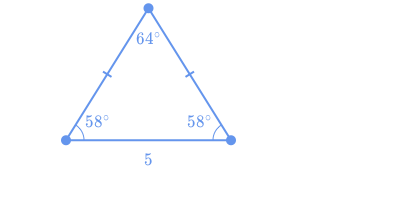
\includegraphics[scale=\shrinkfactor]{figures/4af5c292b250f14e2725fbff73825f6e41348a27.png}



\medskip
\noindent
\textbf{Tags:} {\footnotesize Constructing triangles, CC.7.G.A.2}\\
\textbf{Version:} \DIFdelbegin \DIFdel{5ba2ed08.. 2013-10-17
}\DIFdelend \DIFaddbegin \DIFadd{7d6f4977.. 2013-10-21
}\DIFaddend \smallskip\hrule





\section{\href{https://www.khanacademy.org/devadmin/content/items/xc40b1278855716df}{xc40b1278855716df}}

\noindent
**Draw a \DIFaddbegin \DIFadd{right }\DIFaddend triangle with side lengths $3$, $4$ and $5$.** 

\DIFdelbegin \DIFdel{**Given these criteria is the triangle unique }\DIFdelend \DIFaddbegin \DIFadd{**Is there a unique triangle that satisfies the given conditions}\DIFaddend ?**
[[? interactive-graph 1]]

\paragraph{Ans} 

\fbox{ Yes

}

 No



\paragraph{Hint 1}Let�s start by drawing. We know the lengths of all \DIFdelbegin \DIFdel{$3$ }\DIFdelend \DIFaddbegin \DIFadd{three }\DIFaddend sides. How many triangles can we draw?

\paragraph{Hint 2}The triangle with side lengths $\blue3$, $\blue4$ and $\blue5$ is a right triangle. Since we are given the measures of \DIFdelbegin \DIFdel{$3$ }\DIFdelend \DIFaddbegin \DIFadd{three }\DIFaddend sides, we can draw only \DIFdelbegin \DIFdel{$1$ }\DIFdelend \DIFaddbegin \DIFadd{one }\DIFaddend triangle. 

\paragraph{Hint 3}The triangle is unique.


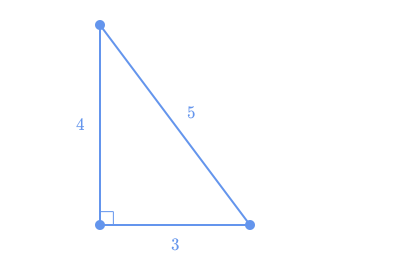
\includegraphics[scale=\shrinkfactor]{figures/758d66a2a3006feaf0b6d196067ab8a9e5a4c587.png}



\medskip
\noindent
\textbf{Tags:} {\footnotesize Constructing triangles, CC.7.G.A.2}\\
\textbf{Version:} \DIFdelbegin \DIFdel{b5262e6e.. 2013-10-17
}\DIFdelend \DIFaddbegin \DIFadd{3adc68e6.. 2013-10-21
}\DIFaddend \smallskip\hrule





\DIFdelbegin \section{}
\addtocounter{section}{-1}
\DIFdel{**Draw an obtuse triangle with angles $45^\circ$,  $35^\circ$ and $100^\circ$.**
}
\DIFdel{**Given these criteria is the triangle unique?**
}\DIFdel{? interactive-graph 1}
\paragraph{\DIFdel{Ans}} 
\addtocounter{paragraph}{-1}
\DIFdel{Yes
}
\DIFdel{\fbox{ No }
}
\paragraph{\DIFdel{Hint 1}}\addtocounter{paragraph}{-1}\DIFdel{Let�s start by drawing. While keeping one angle constant, we can change the side lengths to create one of the other two angles.
}
\DIFdel{For example, while keeping a $\blue{45^\circ}$ angle, we can change the side lengths to create the $\blue{35^\circ}$ angle. The third angle will have measure $\blue{100^\circ}$.
}
\paragraph{\DIFdel{Hint 2}}\addtocounter{paragraph}{-1}\DIFdel{We know the measure of $3$ angles but not the length of any side. We can therefore draw many triangles of the same shape but with different sizes.
}

\paragraph{\DIFdel{Hint 3}}\addtocounter{paragraph}{-1}\DIFdel{The triangle is not unique.
}
\textbf{\DIFdel{Tags:}} \DIFdel{Constructing triangles, CC.7.G.A.2}\textbf{\DIFdel{Version:}} \DIFdel{71b1e27f.. 2013-10-20
}
\DIFdelend \section{\href{https://www.khanacademy.org/devadmin/content/items/xdba9a2b900c8bbcd}{xdba9a2b900c8bbcd}}

\noindent
**How many triangles can be drawn with side lengths $1$, $2$ and \DIFdelbegin \DIFdel{$3$}\DIFdelend \DIFaddbegin \DIFadd{$4$}\DIFaddend ?**

\paragraph{Ans} 

\fbox{ None

}

 Only one

More than one



\paragraph{Hint 1}A triangle is a plane figure with \DIFdelbegin \DIFdel{$3$ }\DIFdelend \DIFaddbegin \DIFadd{three }\DIFaddend straight sides and \DIFdelbegin \DIFdel{$3$ }\DIFdelend \DIFaddbegin \DIFadd{three }\DIFaddend angles. Can we satisfy the definition given the conditions? Let's try to draw a triangle given the conditions.

\paragraph{Hint 2}In general, \DIFdelbegin \DIFdel{the longest }\DIFdelend \DIFaddbegin \DIFadd{any }\DIFaddend side of a triangle \DIFdelbegin \DIFdel{must be }\DIFdelend \DIFaddbegin \DIFadd{is always }\DIFaddend shorter than the sum of the \DIFdelbegin \DIFdel{two other }\DIFdelend \DIFaddbegin \DIFadd{other two }\DIFaddend sides. Because \DIFdelbegin \DIFdel{$\blue{1}+\blue{2} =\blue{3}$}\DIFdelend \DIFaddbegin \DIFadd{$\blue{4} >\blue{2}+\blue{1}$}\DIFaddend , the two sides \DIFdelbegin \DIFdel{$\blue{1}$ and }\DIFdelend $\blue{2}$ \DIFaddbegin \DIFadd{and $\blue{1}$ }\DIFaddend cannot meet to form a third angle \DIFdelbegin \DIFdel{. }\DIFdelend \DIFaddbegin \DIFadd{over the third side $\blue{4}$. 
}


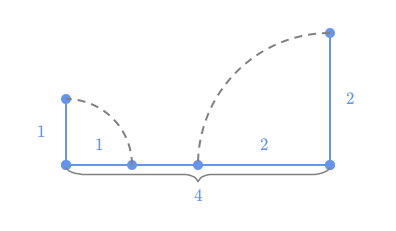
\includegraphics[scale=\shrinkfactor]{figures/dbd401421f460f804da516fa3a58107492fea141.png}

\DIFaddend We cannot create \DIFdelbegin \DIFdel{$3$ }\DIFdelend \DIFaddbegin \DIFadd{three }\DIFaddend angles to satisfy the definition of a triangle.

\DIFdelbegin 
\DIFdelend \paragraph{Hint 3}Given the conditions, no triangles can be drawn.



\medskip
\noindent
\textbf{Tags:} {\footnotesize Constructing triangles, CC.7.G.A.2}\\
\textbf{Version:} \DIFdelbegin \DIFdel{2feadc91.. 2013-10-18
}\DIFdelend \DIFaddbegin \DIFadd{950a8286.. 2013-10-21
}\DIFaddend \smallskip\hrule





\section{\href{https://www.khanacademy.org/devadmin/content/items/xe06107bc78ca0b3c}{xe06107bc78ca0b3c}}

\noindent
**How many triangles can we draw with angles $30^\circ$,  $50^\circ$ and $100^\circ$?**

\paragraph{Ans} 

None

Only one

\fbox{ More than one

}

 

\paragraph{Hint 1}A triangle is a plane figure with \DIFdelbegin \DIFdel{$3$ }\DIFdelend \DIFaddbegin \DIFadd{three }\DIFaddend straight sides and \DIFdelbegin \DIFdel{$3$ }\DIFdelend \DIFaddbegin \DIFadd{three }\DIFaddend angles. The \DIFdelbegin \DIFdel{$3$ }\DIFdelend \DIFaddbegin \DIFadd{three }\DIFaddend angles measures must add up to $\pink{180^\circ}$. Let's add together the angles $\blue{30}^\circ$,  $\blue{50}^\circ$ and $\blue{100}^\circ$:

\begin{align*} 
\text{total angle measure} &= \blue{30^\circ}+\blue{50^\circ}+\blue{180^\circ}\\
&=\pink{180^\circ}
\end{align*}

So, at least \DIFdelbegin \DIFdel{$1$ }\DIFdelend \DIFaddbegin \DIFadd{one }\DIFaddend triangle exists. Let's draw\DIFdelbegin \DIFdel{it}\DIFdelend .

\paragraph{Hint 2}We know the measure of \DIFdelbegin \DIFdel{$3$ }\DIFdelend \DIFaddbegin \DIFadd{three }\DIFaddend angles but not the length of any side. We can draw many triangles with the same shape but different sizes.


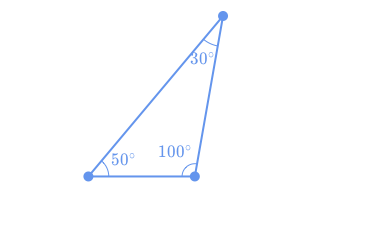
\includegraphics[scale=\shrinkfactor]{figures/cfa8c2afddab68081b192038f3130d47880b443e.png}

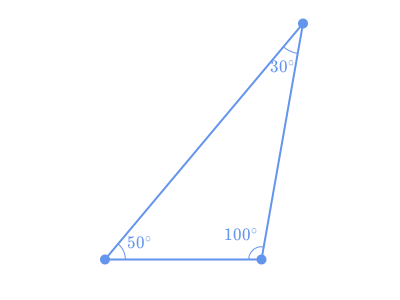
\includegraphics[scale=\shrinkfactor]{figures/b1683148f0f59becb3f7ee5221cd130e632609d7.png}

\paragraph{Hint 3}When only the measures of all \DIFdelbegin \DIFdel{$3$ }\DIFdelend \DIFaddbegin \DIFadd{three }\DIFaddend angles are known, more than one triangle can be drawn.



\medskip
\noindent
\textbf{Tags:} {\footnotesize Constructing triangles, CC.7.G.A.2}\\
\textbf{Version:} \DIFdelbegin \DIFdel{089fe1ab.. 2013-10-20
}\DIFdelend \DIFaddbegin \DIFadd{7c205db7.. 2013-10-21
}\DIFaddend \smallskip\hrule





\section{\href{https://www.khanacademy.org/devadmin/content/items/xe937d430ba8d75d8}{xe937d430ba8d75d8}}

\noindent
**How many triangles can we draw that have one angle measure equal to $45^\circ$ and one side of length $5$?**

\paragraph{Ans} 

None

Only one

\fbox{ More than one

}

 

\paragraph{Hint 1}A triangle is a plane figure with \DIFdelbegin \DIFdel{$3$ }\DIFdelend \DIFaddbegin \DIFadd{three }\DIFaddend straight sides and \DIFdelbegin \DIFdel{$3$ }\DIFdelend \DIFaddbegin \DIFadd{three }\DIFaddend angles. 

The \DIFdelbegin \DIFdel{$3$ }\DIFdelend \DIFaddbegin \DIFadd{three }\DIFaddend angles measures always add up to $\pink{180^\circ}$. We only know \DIFdelbegin \DIFdel{$1$ }\DIFdelend \DIFaddbegin \DIFadd{one }\DIFaddend angle is $\blue{45^\circ}$. We can't find the measures of the other \DIFdelbegin \DIFdel{$2$ }\DIFdelend \DIFaddbegin \DIFadd{two }\DIFaddend angles.

\paragraph{Hint 2}We know the length of only \DIFdelbegin \DIFdel{$1$ }\DIFdelend \DIFaddbegin \DIFadd{one }\DIFaddend side is $\blue5$. Depending if we place the side of length $\blue5$ next to or across from the $\blue{45^\circ}$ angle, we can  draw many triangles with different shapes and different sizes.


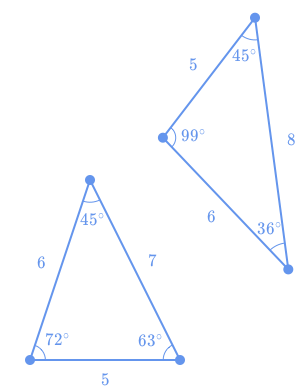
\includegraphics[scale=\shrinkfactor]{figures/8fd2ab6db3cbbe9cbdf43af4cf872835fa89ecf2.png}

\paragraph{Hint 3}If we only know \DIFdelbegin \DIFdel{$1$ angle and $1$ }\DIFdelend \DIFaddbegin \DIFadd{one angle and one }\DIFaddend side length, more than one triangle can be drawn.



\medskip
\noindent
\textbf{Tags:} {\footnotesize Constructing triangles, CC.7.G.A.2}\\
\textbf{Version:} \DIFdelbegin \DIFdel{ba0688a0.. 2013-10-20
}\DIFdelend \DIFaddbegin \DIFadd{e1956610.. 2013-10-21
}\DIFaddend \smallskip\hrule





\section{\href{https://www.khanacademy.org/devadmin/content/items/xf51994a651ca1d7f}{xf51994a651ca1d7f}}

\noindent
**Draw a triangle with angles $30^\circ$,  $50^\circ$ and $100^\circ$.**

\DIFdelbegin \DIFdel{**Given these criteria is the triangle unique }\DIFdelend \DIFaddbegin \DIFadd{**Is there a unique triangle that satisfies the given conditions}\DIFaddend ?**
[[? interactive-graph 1]]

\paragraph{Ans} 

Yes

\fbox{ No

}

 

\paragraph{Hint 1}Let�s start by drawing. While keeping \DIFdelbegin \DIFdel{$1$ }\DIFdelend \DIFaddbegin \DIFadd{one }\DIFaddend angle, we can change the side lengths to create \DIFdelbegin \DIFdel{$1$ }\DIFdelend \DIFaddbegin \DIFadd{one }\DIFaddend of the other \DIFdelbegin \DIFdel{$2$ }\DIFdelend \DIFaddbegin \DIFadd{two }\DIFaddend angles.

While keeping a $\blue{100^\circ}$ angle, we can change the side lengths to create the $\blue{50^\circ}$ angle. The final angle will be $\blue{30^\circ}$.

\paragraph{Hint 2}We know the measure of \DIFdelbegin \DIFdel{$3$ }\DIFdelend \DIFaddbegin \DIFadd{three }\DIFaddend angles but not the length of any side. We can draw many triangles of same shape but different sizes.

\paragraph{Hint 3}The triangle is not unique.

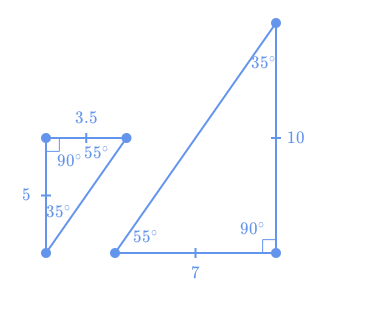
\includegraphics[scale=\shrinkfactor]{figures/13ed90e8845185b7c961687bdf49c22135f67ec5.png}



\medskip
\noindent
\textbf{Tags:} {\footnotesize Constructing triangles, CC.7.G.A.2}\\
\textbf{Version:} \DIFdelbegin \DIFdel{ac2e7f53.. 2013-10-18
}\DIFdelend \DIFaddbegin \DIFadd{d7e4aa43.. 2013-10-21
}\DIFaddend \smallskip\hrule





\section{\href{https://www.khanacademy.org/devadmin/content/items/xf9872931929ac56c}{xf9872931929ac56c}}

\noindent
**Draw a \DIFaddbegin \DIFadd{right }\DIFaddend triangle with side lengths $5$, $12$ and $13$.** 

\DIFdelbegin \DIFdel{**Given these criteria is the triangle unique }\DIFdelend \DIFaddbegin \DIFadd{**Is there a unique triangle that satisfies the given conditions}\DIFaddend ?**
[[? interactive-graph 1]]

\paragraph{Ans} 

\fbox{ Yes

}

 No



\paragraph{Hint 1}Let�s start by drawing. We know the lengths of all \DIFdelbegin \DIFdel{$3$ }\DIFdelend \DIFaddbegin \DIFadd{three }\DIFaddend sides. How many \DIFaddbegin \DIFadd{right }\DIFaddend triangles can we draw?

\paragraph{Hint 2}Since we are given the lengths of all \DIFdelbegin \DIFdel{$3$ }\DIFdelend \DIFaddbegin \DIFadd{three }\DIFaddend sides, we can draw only one \DIFdelbegin \DIFdel{triangle.
}

\DIFdel{Note the triangle }\DIFdelend \DIFaddbegin \DIFadd{right triangle }\DIFaddend with side lengths $\blue5$, $\blue{12}$ and $\blue{13}$\DIFdelbegin \DIFdel{is a right triangle}\DIFdelend .


\DIFaddbegin 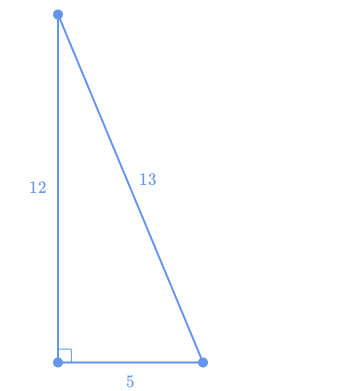
\includegraphics[scale=\shrinkfactor]{figures/227ab289b1de518857460dab83b70e050be9fa46.png}

\DIFaddend \paragraph{Hint 3}The triangle is unique.



\medskip
\noindent
\textbf{Tags:} {\footnotesize Constructing triangles, CC.7.G.A.2}\\
\textbf{Version:} \DIFdelbegin \DIFdel{81990b3f.. 2013-10-20
}\DIFdelend \DIFaddbegin \DIFadd{ba30b682.. 2013-10-21
}\DIFaddend \smallskip\hrule





\end{document}
